\documentclass[../AnalysisNoteJBuxton.tex]{subfiles}
\begin{document}

\subsection{V0 Selection}
\label{V0Selection}

$\Lambda$ ($\bar{\Lambda}$) and K$^{0}_{S}$ are neutral particles which cannot be directly detected, but must instead be reconstructed through detection of their decay products, or daughters.  
This process is illustrated in Figure \ref{fig:V0Reconstruction}.
In general, particles which are topologically reconstructed in this fashion are called V0 particles.
The class AliFemtoV0TrackCutNSigmaFilter (which is an extension of AliFemtoV0TrackCut) is used to reconstruct the V0s.

\begin{figure}[h]
  \centering
  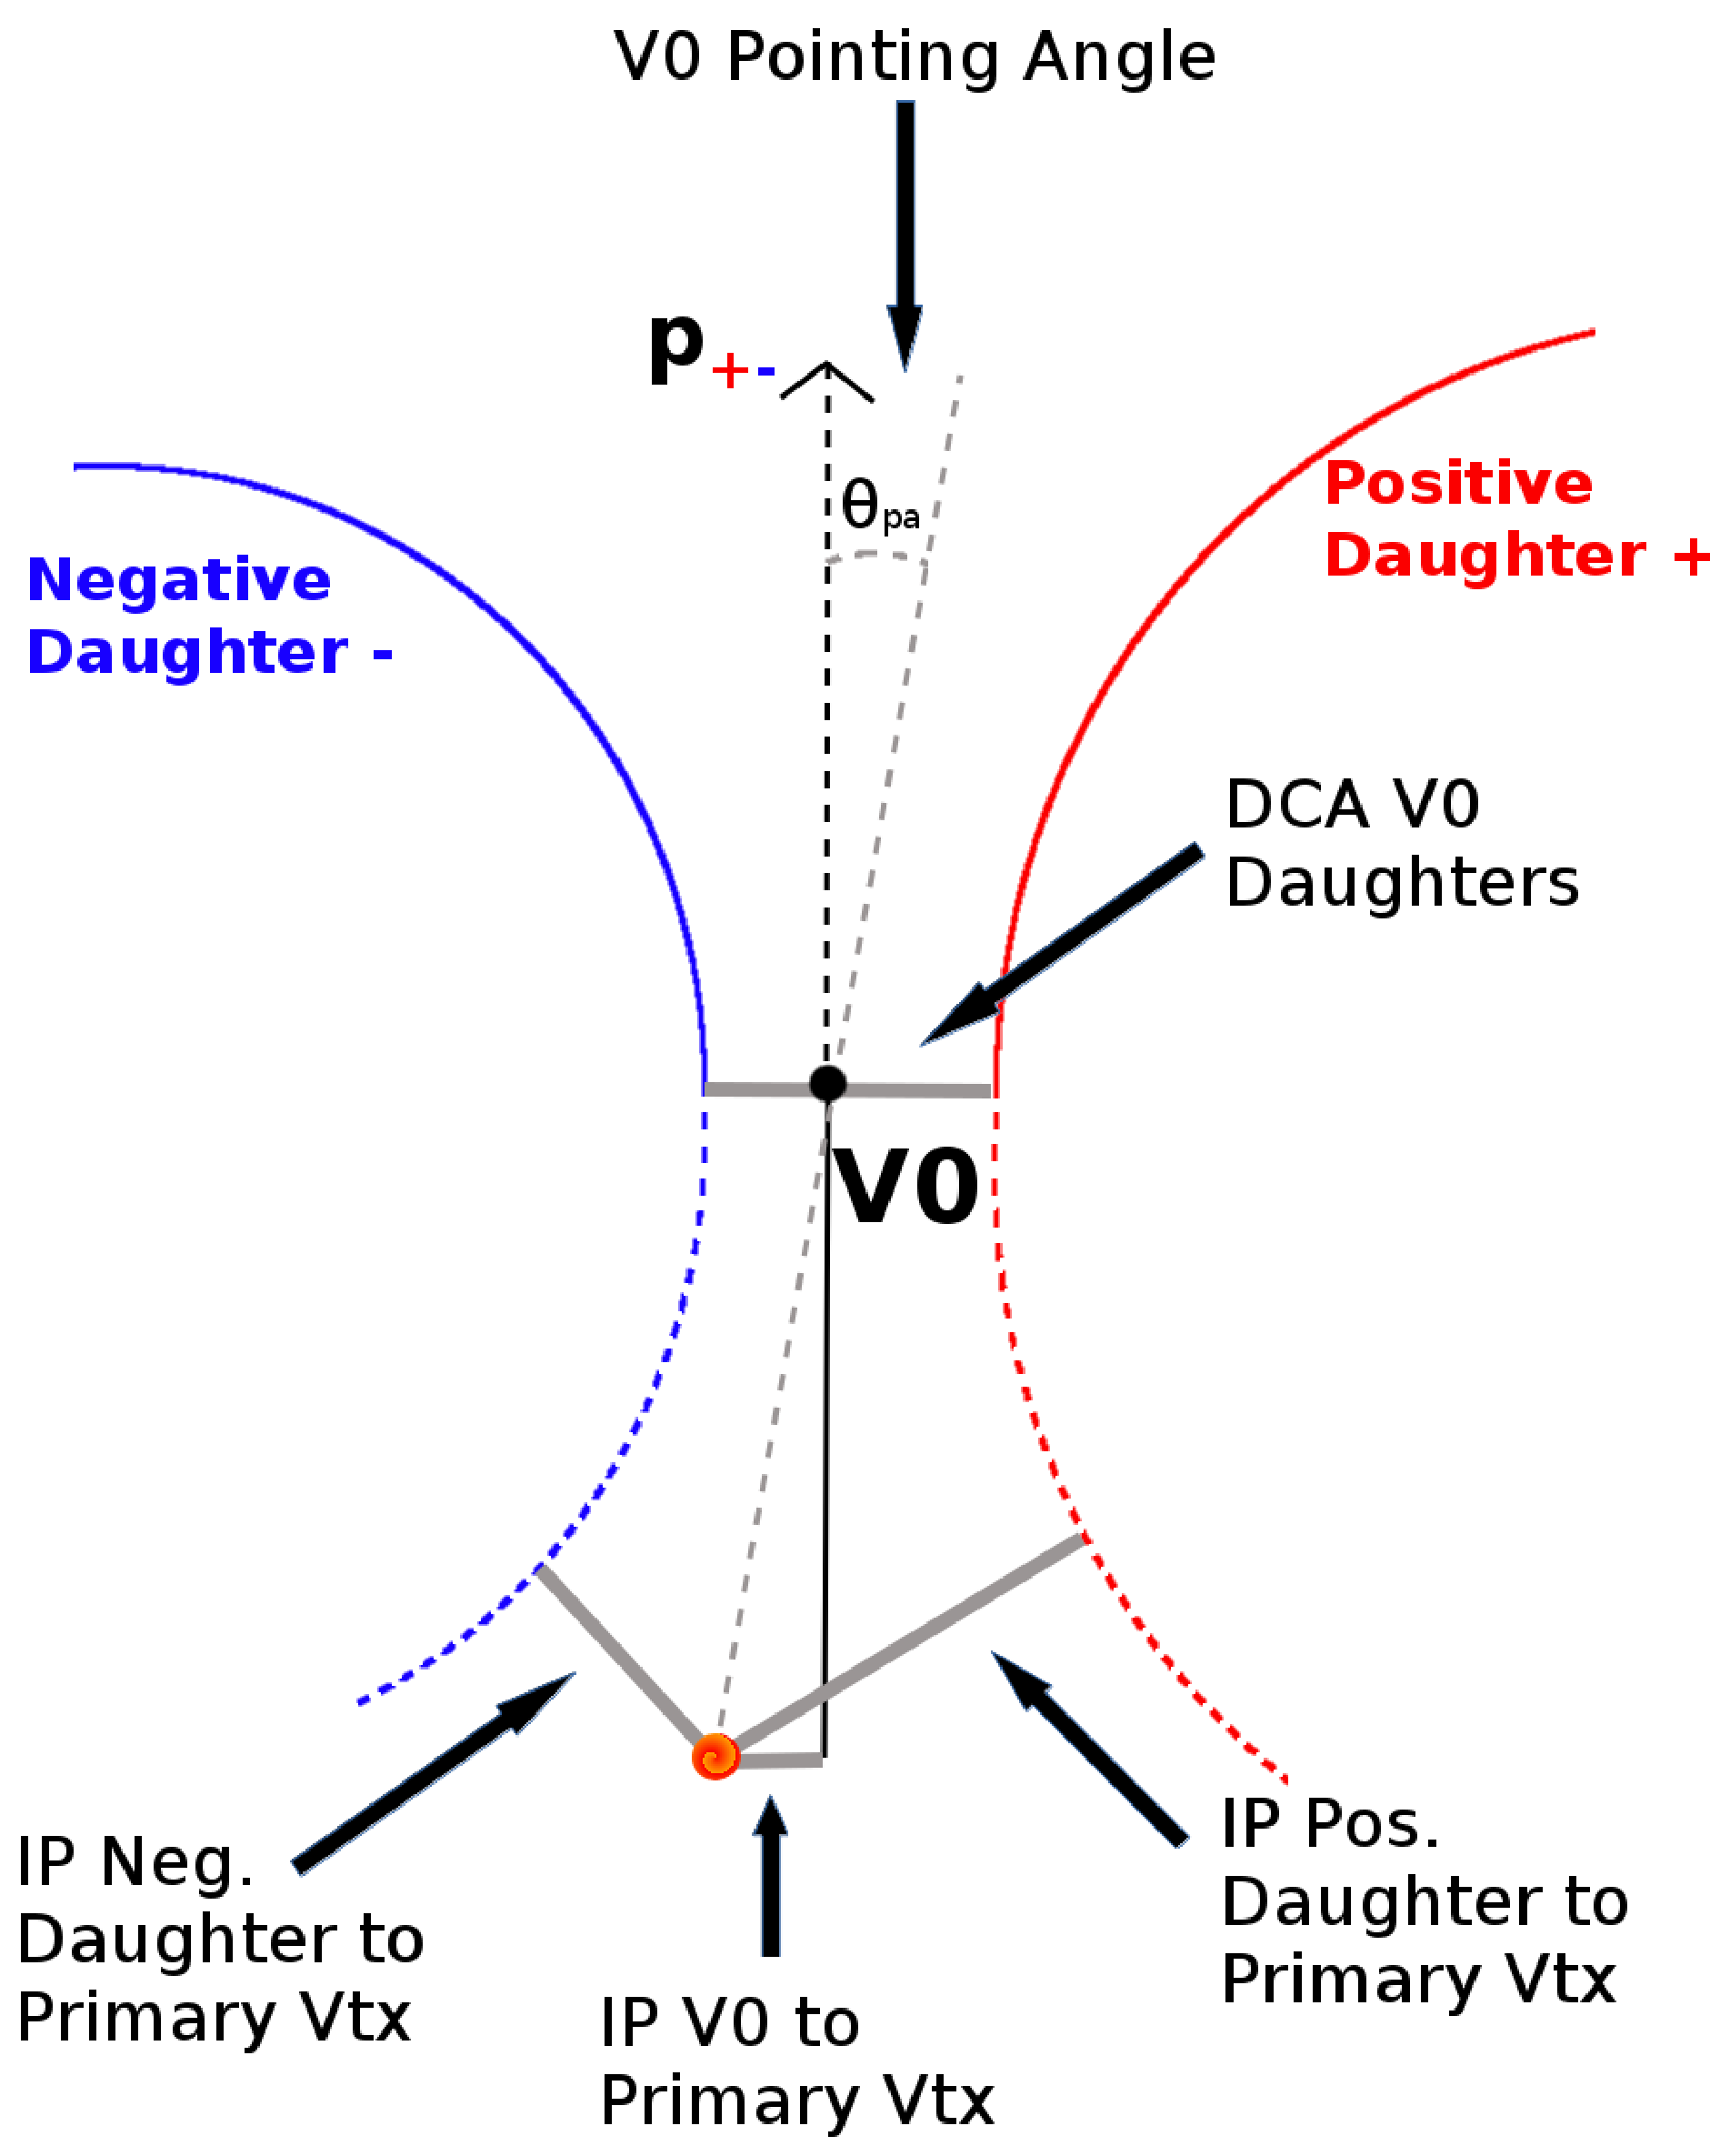
\includegraphics[width=0.5\textwidth]{3_DataSelection/Figures/V0CutsGeneral.pdf}
  \caption[V0 Reconstruction]{V0 Reconstruction}
  \label{fig:V0Reconstruction}
\end{figure}

\subfile{3_DataSelection/3.3.1_LambdaReconstruction.tex}
\subfile{3_DataSelection/3.3.2_K0sReconstruction.tex}

\end{document}
